\section{Why agents change the scheduling problem}
\label{sec:agents}
\subsection{A session is a sequence of dependent visits}
For session $i$, let turn $k$ contain queueing $Q_{ik}$, inference $I_{ik}$,
tool time $Z_{ik}$, and other orchestration $O_{ik}$. A sequential job has
\begin{equation}
 J_i=\sum_k(Q_{ik}+I_{ik}+Z_{ik}+O_{ik}).
 \label{eq:job}
\end{equation}
Parallel tools replace some sums with critical-path expressions. A fast
individual LLM call does not guarantee fast $J_i$, and a policy that improves
mean request latency can still harm long multi-turn jobs. Conversely, if tools
dominate and inference is already fast, substantial GPU acceleration may barely
change completion time.

\fig{agent}{0.97}{One cycle of an agent session. The tool gap is both a source of
uncertainty and an opportunity to prepare state. An unchanged old prefix may
remain reusable when a new observation is appended, subject to exact identity.}{agent}

In a stationary closed population of $N$ sequential sessions with mean inference
visit response $R$ and non-inference think/tool time $Z$, the interactive
response-time relation is $X=N/(R+Z)$ visits per second. This follows by counting
one completed cycle per session per average cycle duration. Increasing engine
speed reduces $R$ and can increase the rate of future arrivals. Replaying fixed
request timestamps misses this feedback. Admission delays also shift future
returns, so the workload is partly affected by the policy being evaluated.

AgentSysBench's 2026 preprint studies ten agentic applications and reports
heterogeneous bottlenecks, substantial non-LLM costs, and retained state across
idle intervals~\cite{agentbench}. This supports measuring complete workflows;
it does not prove that all agents have the same return-time distribution.
MLCommons' July 2026 agentic-inference announcement similarly emphasizes growing
context and dependent multi-turn execution~\cite{mlperf}. A benchmark proposal
or announcement must not be confused with a completed, universally adopted
performance standard.

\subsection{Queueing: why small demand errors matter near saturation}
For a deliberately simple M/M/1 system with Poisson arrivals, exponential
service, one server, and utilization $\rho=\lambda/\mu<1$,
\begin{equation}
 \E[R]=\frac{1}{\mu-\lambda}
       =\frac{1/\mu}{1-\rho}.
 \label{eq:mm1}
\end{equation}
At utilization 0.5, mean response is twice mean service; at 0.9 it is ten times;
at 0.99 it is one hundred times. A batched GPU system is not M/M/1, but this
example explains why headroom and bursts matter. Mean capacity alone cannot
predict tail latency when the service process changes with batching and state.

\fig{queueing}{0.90}{Analytical queueing illustration. The steep rise near
saturation motivates controlling overload; it is not an empirical fit to ATFM,
vLLM, or a real GPU.}{queueing}

If a resource has capacity $C_r$ work units per second and arrival work demand
$\lambda\E[D_r]$, a necessary long-run stability condition is
$\lambda\E[D_r]<C_r$. The resource may be compute, link bytes, CPU time, or
storage IO. Memory is also a stock constraint: instantaneous occupancy must
fit, not just average allocation rate. Holding background work can shift peaks;
it cannot make permanently excessive admitted work disappear. Rejection,
additional capacity, or a lower work budget is eventually necessary.

A useful policy must state whose latency it improves. Giving all interactive
traffic priority can starve background jobs. A finite delay cap protects
background progress but may force release into an already overloaded system.
Thus bounded delay and unconditional overload avoidance cannot both be promised
under arbitrary arrivals. This is a policy tradeoff, not an implementation bug.

\subsection{Forecasting the remaining tool time}
Let $T$ be a tool's total duration, $a$ its elapsed age, and $\mathcal I_t$ the
information available now. With survival function $S(x)=\Prb(T>x)$, the
age-conditioned residual distribution is
\begin{equation}
 \Prb(T-a\le h\mid T>a)=1-\frac{S(a+h)}{S(a)},\quad S(a)>0.
 \label{eq:residual}
\end{equation}
A tool that has already run for 60 seconds is not a fresh draw from its original
duration distribution. Heavy tails can make expected remaining time increase
with age; the memoryless exponential is a special case. Completed-only training
can also bias estimates when long-running calls are censored by observation
windows or cancellation.

Progress can provide additional evidence. If a tool reports completed work $c$
out of total $w$ at uncertain rate $V$, a simple remaining-time model is
\begin{equation}
 R=\frac{w-c}{V}+R_{\mathrm{finalize}}.
\end{equation}
This is a model, not a universal parser truth. Work units may change cost over
time; setup/finalization may dominate; multiple stages can reset counters; a
reported percentage can be nonlinear. A robust system should retain uncertainty
and detect invalid or stale progress rather than extrapolate one point as a
certain completion timestamp.

For a concrete illustration, two tools have both run 20 seconds. One reports
950 of 1000 uniform items completed at a stable 50 items/s; the other reports
100 of 1000 at 5 items/s. The naive residual point estimates are one second and
180 seconds before finalization. Age alone cannot distinguish them. Whether
this extra distinction is actionable depends on cache size, transfer lead time,
and forecast reliability.

\subsection{From return times to fleet demand}
Let $R_i$ be the next return time relative to now and $D_{ir}$ the resource demand
of that return. A simplified cumulative demand process is
\begin{equation}
 A_r(h)=\sum_{i=1}^N D_{ir}\ind\{R_i\le h\}+A_{r,\mathrm{new}}(h).
 \label{eq:demand}
\end{equation}
An actual agent can return several times within a long horizon, requiring a
multi-visit model. The one-return form makes the distinction between timing and
size explicit. Forecasting only request count misses long prompts and large
contexts; forecasting only mean bytes misses synchronized return bursts.

In general,
\begin{equation}
 \E[D_{ir}\ind\{R_i\le h\}]
 \ne \E[D_{ir}]\Prb(R_i\le h)
\end{equation}
unless the relevant conditional independence holds. Slow tools can produce
larger observations. Backend congestion can correlate many sessions' durations.
Monte Carlo samples should preserve such dependencies when supported by data.
For indicator returns with equal demand $d$,
\begin{equation}
 \operatorname{Var}(A)=d^2\!\left[\sum_i p_i(1-p_i)
 +2\sum_{i<j}\operatorname{Cov}(\ind_i,\ind_j)\right].
\end{equation}
Assuming independence deletes the covariance term and can understate tail risk.
A forecast should be evaluated under shared backend stalls and release bursts,
not only independently overlaid sessions.

Cumulative arriving KV demand is not instantaneous resident memory. Occupancy
also depends on completion, eviction, sharing, output growth, and placement.
Converting arrival quantiles into memory safety therefore needs a state/lifetime
model or a deliberately conservative bound. Similarly, a prefill-token capacity
per time slot is a calibrated work proxy, not a hardware invariant.

\subsection{Retention as a decision under uncertainty}
Suppose keeping one session's state until either it returns or timeout $\tau$
avoids miss cost $C$ if it returns in time. Let $F$ be its residual return CDF,
$m$ bytes occupied, and $\lambda_m$ the opportunity cost per byte-second in the
same objective units as $C$. Relative to immediate eviction, a simple expected
net value is
\begin{equation}
 V(\tau)=CF(\tau)-\lambda_m m\E[\min(R,\tau)]
 =CF(\tau)-\lambda_m m\int_0^\tau(1-F(u))\,du.
 \label{eq:retention}
\end{equation}
This assumes constant miss benefit and memory price and ignores interactions,
shared blocks, and capacity discontinuities. It is a useful derivation, not the
algorithm implemented in ATFM. With density $f$,
\begin{equation}
 V'(\tau)=Cf(\tau)-\lambda_m m(1-F(\tau)).
\end{equation}
Where survival is positive, extending retention is locally favorable when
$C h(\tau)>\lambda_m m$, with hazard $h=f/(1-F)$. A point estimate of return
time loses the uncertainty needed for this calculation. Multiple local optima
are possible; a local hazard test alone is not a global optimization method.

\fig{retention}{0.91}{Derived retention value under two assumed memory opportunity
costs. The return distribution is a normal distribution truncated to positive
time. The miss penalty is 200 ms. The illustration shows that a forecast alone
does not determine a retention policy; congestion changes the value of memory.}{retention}

Prefetch has a related timing constraint. If transfer requires lead time $\ell$
and starts $s$ seconds from now, then its probability of completing before reuse
is approximately $\Prb(R\ge s+\ell)$ under a fixed-lead-time model. Starting too
early occupies scarce space and can evict useful state. Starting too late
leaves a demand-path stall. Transfer times themselves can be random and
correlated with the same bursts the policy is trying to manage.

\subsection{The closest prior work}
Continuum's inspected September 2026 revision uses bounded KV retention with a
time-to-live mechanism and program-level scheduling. Its motivation includes
reload/recompute costs, queueing after eviction, and robustness to uncertain
tool duration~\cite{continuum}. It is a direct baseline for a claim about agent
cache retention, not merely background context. An ATFM comparison should use
the actual supported policy or label a simplified reproduction honestly.

\fig{papers/continuum-cache}{1.0}{Continuum's original cache-retention
motivation. Compare the illustrated agent execution and cache lifetimes when
reading its TTL policy. Reproduced from Li et al.~\cite{continuum}, Figure 1,
arXiv:2511.02230v7, CC BY 4.0; scaled and format-converted only.}{continuum-original}

ThunderAgent's June 2026 revision represents agent workflows as programs and
coordinates KV-related scheduling with tool resources and environment
preparation~\cite{thunder}. It already addresses the mismatch between isolated
request decisions and workflow needs. ATFM's possible contribution is a
particular use of conditional forecasts and cross-session uncertainty, not the
idea of treating agents as programs.

\begin{figure}[htbp]
\centering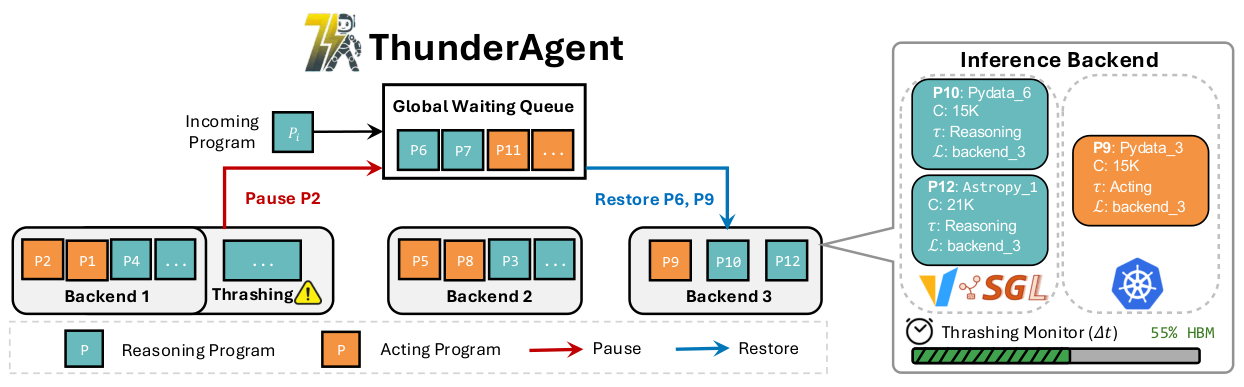
\includegraphics[width=\linewidth]{figures/papers/thunderagent-overview.png}
\caption{ThunderAgent's original system overview, showing program-aware
coordination of inference and tool execution. Reproduced from Kang et
al.~\cite{thunder}, Figure 3, arXiv:2602.13692v3, CC BY 4.0; scaled only.}
\label{fig:thunder-original}
\end{figure}

These systems also bound the research claim. If a simple robust TTL, native
retention priority, or working-set policy captures most of the benefit, a more
complex predictor may not be worth its cost. The right experiment asks what
extra information changes a decision, not whether the system beats an
intentionally oblivious baseline.
